\section{共包协议设计与对照封装}\label{sec:design}

\begin{figure}[t]
  \centering
  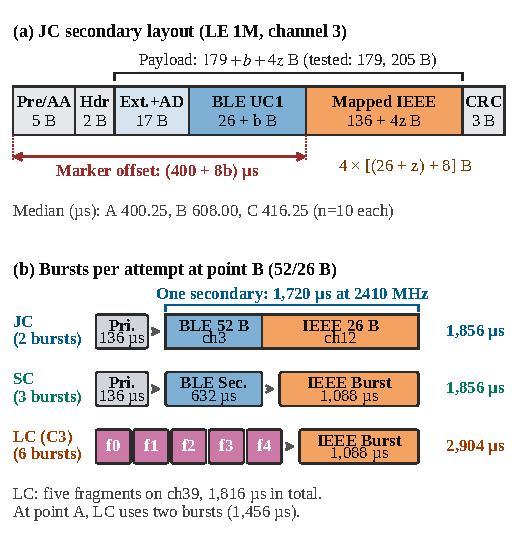
\includegraphics[width=\columnwidth]{fig-uc1-layout-bursts.pdf}
  \caption{统一紧凑格式（\proto{}）共包次信道数据单元布局与单次尝试突发对比：(a) \texttt{AUX\_ADV\_IND} 字节预算与确定性偏移 $\num{400}+8b\,\si{\micro\second}$；(b) B 点（$52/26$\,B）下 \modejc{}、\modesc{} 与需五片 \fragproto{} 分片的 \modelc{} 突发结构。}
  \label{fig:layout}
\end{figure}

\subsection{单发送机封装模式与字节/波形预算}\label{sec:design_modes}

发送机按 \SI{500}{ms} 时隙（$T_{\text{slot}}{=}\SI{500}{ms}$）向 \ble{} 接收链与 \stdfour{} 接收链调度发送尝试；在 P4 中，相邻逻辑任务的起始槽相隔 $6$ 个时隙（\SI{3}{s}）。每项逻辑任务由 $(\texttt{run\_id}, \texttt{command\_id})$ 唯一标识，在单向无确认信道下按固定计划尝试次数 $K$ 或共同单任务波形预算上限 $Q$（\si{\micro\second}）执行开环发送，每次物理尝试占据一个递增槽号 $\texttt{slot\_index}$。如图~\ref{fig:layout} 所示，本文在同一任务语义下实现三种封装模式：共包扩展广播（\modejc{}）每次尝试发射 $2$ 个突发，包括 $1$ 个主信道 \texttt{ADV\_EXT\_IND}（\SI{136}{\micro\second}）与 $1$ 个位于 \ble{} ch3（\SI{2410}{MHz}，与 \stdfour{} ch12 中心频点重合）的次信道 \texttt{AUX\_ADV\_IND}，在单帧中顺次容纳 \ble{} 记录与 BlueBee 映射后的 \stdfour{} 记录；同频分别扩展广播（\modesc{}）每次尝试发射 $3$ 个突发，即主信道指针、仅含 \ble{} 记录的 ch3 次信道帧以及独立的 ch12 BlueBee 映射 \stdfour{} 突发；传统广播/分片基线（\modelc{}）每次尝试发射 $F+1$ 个突发，在传统广播信道 ch39（\SI{2480}{MHz}）发送 $F$ 帧 \ble{} 广播后再于 ch12 发送 $1$ 个独立 \stdfour{} 突发。

在应用记录层，\ble{} 与 \stdfour{} 各自独立封装并校验一条长度为 $(26+n)$\,B 的小端 \proto{} 记录（\ble{} 侧 $n{=}b$，\stdfour{} 侧 $n{=}z$）。每条记录由 \SI{24}{B} 固定头（含 \texttt{magic=0xC1}、显式版本类型字节 \texttt{0x10} 纯时间更新或 \texttt{0x11} 控制命令、\texttt{run\_id}、\texttt{slot\_index}、\texttt{period\_ms}、\texttt{command\_id}、\texttt{target\_id}、\texttt{opcode}、\texttt{arg}、\texttt{valid\_offset\_ms}、\texttt{execute\_offset\_ms} 与 \texttt{extra\_len}）、$n$\,B 本侧扩展净荷以及 \SI{2}{B} \texttt{CRC-16/CCITT-FALSE} 校验构成。在 \modejc{} 冻结布局中，扩展广播头、Flags AD 与 Manufacturer AD 头共占 \SI{17}{B}，BlueBee 映射区占 $4(26+z+8)=136+4z$\,B（内含 \SI{8}{B} \stdfour{} PHY/MAC 封装），故次信道 PDU 载荷长度为
\begin{equation}\label{eq:sec_payload}
  L_{\text{sec}}(b,z) = 17 + (26 + b) + (136 + 4z) = 179 + b + 4z~\text{B}.
\end{equation}
受 \SI{255}{B} 次信道载荷协议上限约束，式~\eqref{eq:sec_payload} 的字节算术边界为 $b+4z\le 76$；本文阶段一冻结工作域限定为 $0\le b\le 26$、$0\le z\le 6$ 且满足共同约束 $b+4z\le 26$（两项边际最大值 $b{=}26$ 与 $z{=}6$ 不可组合）。实验选取三组代表配置（按 \ble{}/\stdfour{} 顺序）：短负载 A 点（扩展 $0/0$\,B，完整记录 $26/26$\,B，次信道载荷 \SI{179}{B}）、长 \ble{} 负载 B 点（扩展 $26/0$\,B，完整记录 $52/26$\,B，载荷 \SI{205}{B}）及双侧非对称负载 C 点（扩展 $2/6$\,B，完整记录 $28/32$\,B，载荷 \SI{205}{B}）；另设 B1 点（扩展 $1/0$\,B，完整记录 $27/26$\,B）核验传统广播 \SI{27}{B} 直接承载边界。

在 LE~1M 速率下，三种模式单次完整逻辑尝试的设计有效波形代理预算（\si{\micro\second}，不含包间静默与调谐保护间隔）如表~\ref{tab:budget} 所示，由下式精确给出：
\begin{align}
  C_{\modejc}(b,z) &= C_{\modesc}(b,z) = 1648 + 8b + 32z,\label{eq:cost_jc_sc}\\
  C_{\modelc}(b,z) &=
  \begin{cases}
    8(182 + b + 4z), & b \le 1,\\
    8(35F + 162 + b + 4z), & b \ge 2.
  \end{cases}\label{eq:cost_lc}
\end{align}
其中 \modelc{} 在 $b\le 1$ 时以单个 Manufacturer AD 直接承载完整 \ble{} 记录（$F{=}1$）；当 $b\ge 2$ 时进入 \fragproto{} 分片，每片含 \SI{20}{B} 传统广播空口封装与 \SI{15}{B} 分片头，最多承载 \SI{12}{B} 记录字节，分片数 $F=\lceil(26+b)/12\rceil$（B 点 $52$\,B 对应 $F{=}5$）。由式~\eqref{eq:cost_jc_sc} 可见，\modejc{} 与 \modesc{} 在任意 $(b,z)$ 下单次提交波形代理预算完全相等，而 \modejc{} 将每次尝试的突发数由 $3$ 次降至 $2$ 次。在同预算上限 $Q$ 策略下，各模式分配计划尝试次数 $K_m=\lfloor Q/C_m\rfloor$，并将剩余未用预算 $Q-K_m C_m$ 显式记录而不以无意义填充补齐。

% ============================================================
%  表 1（中文同步版）：与 ../tables/tab-budget.tex 数值 100% 同步
%  数据源：python/experiments/p5_freeze_20261124/p5_p2_h2_h3.csv
% ============================================================
\begin{table}[t]
\centering
\caption{代表性负载点的字节布局、单尝试提交波形代理预算与有线馈线核验。}
\label{tab:budget}
\setlength{\tabcolsep}{2.0pt}
\scriptsize
\begin{tabular}{@{}lccccccc@{}}
\toprule
\textbf{测点} & \textbf{记录} & \textbf{映射} & \textbf{\modejc{}载荷} & \multicolumn{3}{c}{\textbf{突发数 / 代理 (\si{\micro\second})}} & \textbf{偏移} \\
\cmidrule(lr){5-7}
$(b,z)$ & B/Z & (B) & (B) & \modejc{} & \modesc{} & \modelc{} ($F$) & (\si{\micro\second}) \\
\midrule
A $(0,0)$   & 26/26 & 136 & 179 & 2/\num{1648} & 3/\num{1648} & 2/\num{1456} (1) & 400.25 \\
B1 $(1,0)$  & 27/26 & 136 & 180$^{\mathrm{a}}$ & 2/\num{1656}$^{\mathrm{a}}$ & 3/\num{1656}$^{\mathrm{a}}$ & 2/\num{1464} (1) & --- \\
C $(2,6)$   & 28/32 & 160 & 205 & 2/\num{1856} & 3/\num{1856} & 4/\num{2344} (3) & 416.25 \\
B $(26,0)$  & 52/26 & 136 & 205 & 2/\num{1856} & 3/\num{1856} & 6/\num{2904} (5) & 608.00 \\
\bottomrule
\end{tabular}
\par\smallskip
\raggedright\scriptsize
全部 10 个已测 \texttt{R0} 分支（轮次 2702--2710、2718）均获 $10/10$ 联合解析。$F$ 为传统 \ble{} 帧数/尝试（$b\le 1$ 取 $F{=}1$；$b\ge 2$ 取 $F{=}\lceil(26{+}b)/12\rceil$ 片 \fragproto{} 分片，另加 $1$ 次 \stdfour{} 突发）。$^{\mathrm{a}}$公式值；B1 点仅采集 \SI{27}{B} 直接 \modelc{} 上限（轮次 2710）。同 IQ 偏移中位数（每点 $n{=}10$）核验 $400{+}8b\,\si{\micro\second}$，不代表跨设备时钟误差。
\end{table}


\subsection{确定性包内偏移、重发语义与 \fragproto{} 状态机}\label{sec:design_semantics}

\proto{} 将时隙计划参考定义为 $\texttt{ref\_tick\_ms}=\texttt{slot\_index}\times\texttt{period\_ms}$，在共包模式下绑定于次信道 \ble{} 前导码起点。由于次信道帧在前导码与接入地址（\SI{5}{B}）、PDU 头（\SI{2}{B}）、扩展/AD 头（\SI{17}{B}）及 \ble{} 记录（$26+b$\,B）之后即进入 BlueBee 映射区（始于载荷偏移 $43+b$ 字节），\ble{} 前导码至 \stdfour{} 参考标记的理论结构偏移为
\begin{equation}\label{eq:offset}
  \Delta t_{\text{marker}}(b) = (5 + 2 + 43 + b) \times \SI{8}{\micro\second} = 400 + 8b~\si{\micro\second}.
\end{equation}
为将每侧固定记录开销维持在 \SI{26}{B}，\stdfour{} 侧依赖轮次前预共享配置中的 $b$ 值实施该包内位置补偿，而不能从自身 $(26+z)$\,B 记录推导对侧长度；若缺失匹配布局配置或配置校验失败，接收机仍可记录本侧有效命令，但强制置 $\texttt{timing\_eligible}=\text{false}$，禁止静默套用旧版固定偏移。

在计划的 $K$ 次开环尝试中，各侧应用命令内容及绝对有效截止时刻 $V=\texttt{ref\_tick\_ms}+\texttt{valid\_offset\_ms}$、目标软件处理时刻 $E=\texttt{ref\_tick\_ms}+\texttt{execute\_offset\_ms}$（满足 $\texttt{ref\_tick\_ms}\le V<E$）均保持不变；每次尝试写入各自的 $\texttt{slot\_index}$、重新计算的相对时间偏移并更新记录 CRC，防止重发不断推迟截止期。若同一任务在不同尝试中出现目标、操作码、净荷或恢复后 $V/E$ 冲突，尚未处理的挂起任务立即取消且后续即使恢复原参数也不得重新接受或更新时间模型。纯时间更新槽（\texttt{0x10}）将命令字段与偏移全部置零，但保持与本轮配置一致的扩展填充长度以维持式~\eqref{eq:offset} 位置不变；其发射计入总波形成本，但不增加逻辑任务分母。

针对 \modelc{} 在 $b\ge 2$ 时的跨尝试分片混拼风险，\fragproto{}（\texttt{magic=0xC3}）采用 \SI{15}{B} 分片头（含版本、\texttt{run\_id}、\texttt{slot\_index}、\texttt{command\_id}、分片索引、总片数与总记录长度）加 \SIrange{1}{12}{B} 记录字节，按 $(\texttt{AdvA}, \texttt{run\_id}, \texttt{slot\_index}, \texttt{command\_id})$ 实施槽隔离重组，禁止跨尝试拼接。重组器为并发收集队列 \texttt{pending} 与已关闭墓碑表 \texttt{closed} 分配独立容量上限，并强制维持容量预留不变量 $\lvert\texttt{closed}\rvert+\lvert\texttt{pending}\rvert\le\texttt{closed\_limit}$：已关闭身份保留至轮次显式结束而不做 LRU 淘汰，新尝试进入 \texttt{pending} 前必须预留未来 \texttt{closed} 槽位，避免释放后旧分片复活已关闭尝试；重组完成后仍须复核记录级 \texttt{app\_crc16}、版本、长度及标识字段与分片头完全一致，方可提交任务去重层。
